\documentclass{beamer}

% Used packages
\usepackage{graphicx}
\usepackage{hyperref}
\usepackage{algorithm}
\usepackage{array}
\usepackage{verbatim}
\usepackage{hyperref}
\hypersetup{
    bookmarks=true,    % show bookmarks bar?
    pdftitle={Specification},    % title
    pdfauthor={Selyunin, Pelesic, Jakovljevic},                     % author
    pdfsubject={TeX and LaTeX},                        % subject of the document
    pdfkeywords={TeX, LaTeX, graphics, images}, % list of keywords
    colorlinks=false,       % false: boxed links; true: colored links
    linkcolor=blue,       % color of internal links
    citecolor=black,       % color of links to bibliography
    filecolor=black,        % color of file links
    urlcolor=purple,        % color of external links
%    linktoc=page            % only page is linked
}

%\usepackage{algpseudocode}
    \renewcommand{\arraystretch}{1.8}
% The title
\title[Code Mobility]{Code Mobility}

% The date
\date{06. December 2012}

% The author
\author[Selyunin,Pelesi\'c,Jakovljevi\'c]{
 \Large{Konstantin Selyunin}\\
  \small{\texttt{e1228206@student.tuwien.ac.at}}\\
 \Large{Igor Pelesi\'c}\\
  \small{\texttt{igor.pelesic@gmail.com}}\\
 \Large{Miljenko Jakovljevi\'c}\\
  \small{\texttt{micky686@gmail.com}}\\
}

% Use Warsaw theme
\usetheme{Warsaw}

% New commands
\newcommand{\mc}[1]{$\mathcal{#1}$}

\theoremstyle{definition} \newtheorem{mdefinition}{Definition}
\theoremstyle{plain} \newtheorem{mtheorem}{Theorem}
\theoremstyle{plain} \newtheorem{mcorollary}{Corollary}
\theoremstyle{plain} \newtheorem{mfact}{Fact}

% Begin of document
\begin{document}

\begin{frame}
	\titlepage
\end{frame}

\begin{frame}
	\frametitle{Outline}
	\tableofcontents
\end{frame}

\section{Introduction}


\subsection{Code mobility overview}
\begin{frame}
	\frametitle{Code mobility overview}
 		\framesubtitle{Concept of code mobility}
	\begin{block}{Concept of code mobility}
		\begin{description}
			\item	Mobile agent
			\item	{\it Strong} and {\it weak} code mobility
			\item   Layered architecture
		\end{description}
	\end{block}

	\begin{block}{Advantages of code mobility}
		\begin{description}
			\item	Move code close to resources 
			\item	Enable client customization of remote resources
			\item	Performance gains
		\end{description}
	\end{block}	
\cite{10.1109/32.685258, BartocciCMV06} 

%\cite{BartocciCMV06}
\end{frame}

\subsection{Level of abstraction}
\begin{frame}
\frametitle{Level of abstraction}
\begin{centering}
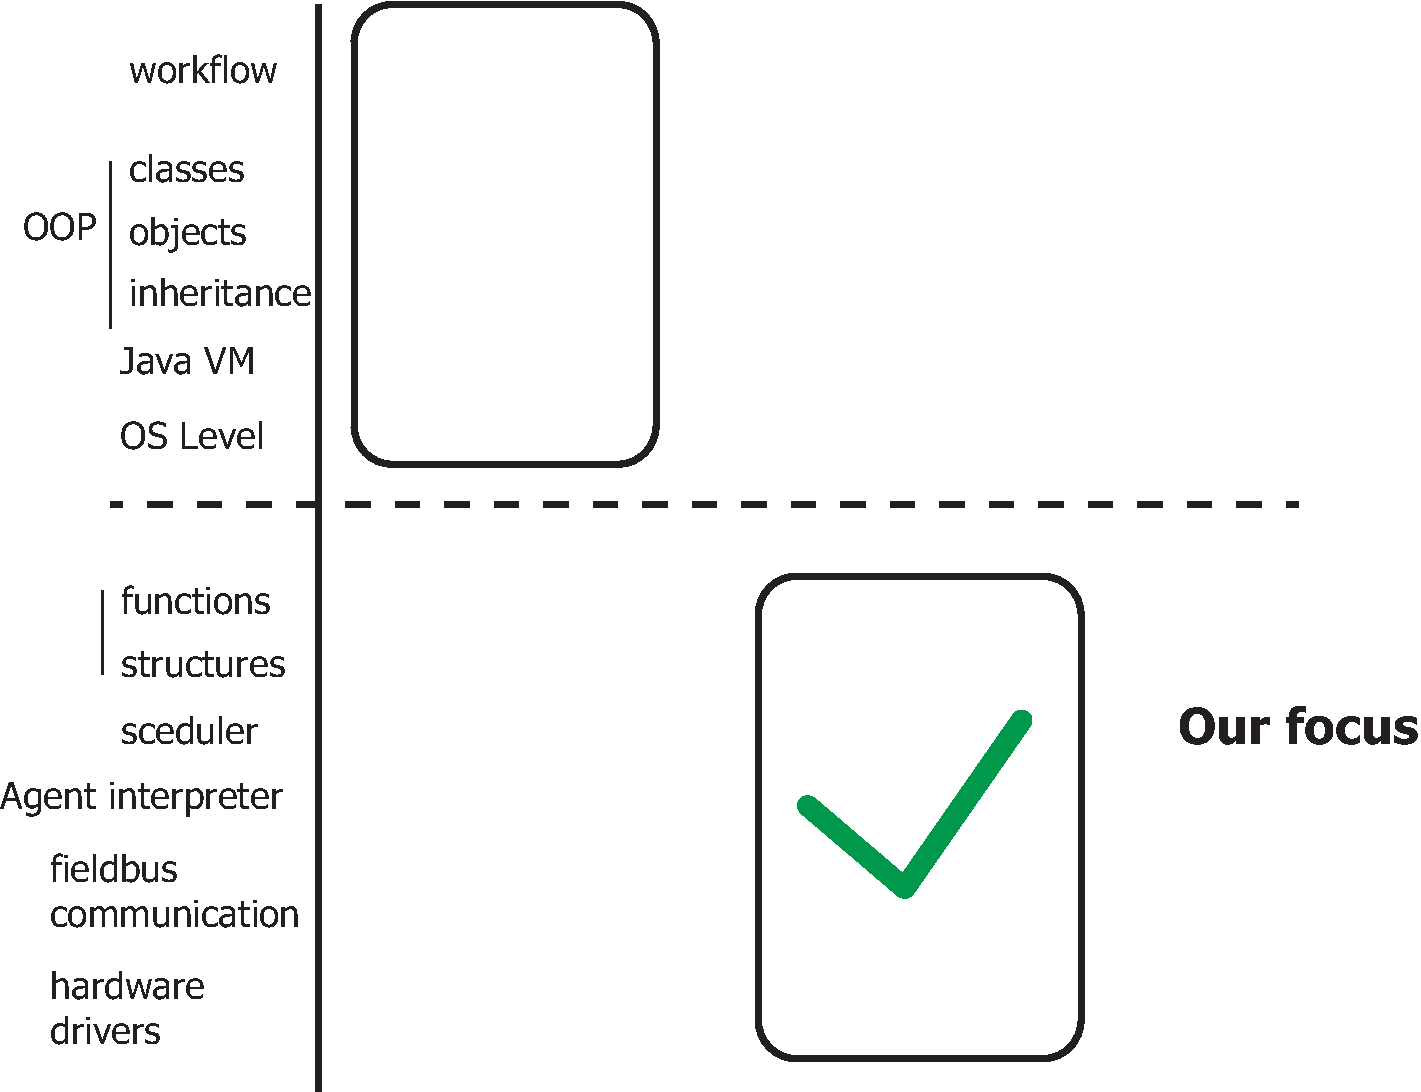
\includegraphics[width=3in]{img/abstraction-3-eps-converted-to.pdf}
\end{centering}
\end{frame}
\begin{comment}
\subsection{Design challenges for the project}
\begin{frame}
\frametitle{Design challenges for the project}
\begin{tabular}{ll}
Processing gap & \\

Performance & \\

Memory management & \\

Communication design & \\
\end{tabular}

\end{frame}
\end{comment}

\subsection{Requirements}
\begin{frame}
	\frametitle{Requirements}
% 	\framesubtitle{}
%To develop a solution that allow to trasfer code from one platform to another

\begin{itemize}
	\item Agents:
	\begin{itemize}
		\item simple language 
		\item support mobility and message exchange
	\end{itemize} 
	\item Platform:
	\begin{itemize}
		\item execute agents concurrently
		\item provide hardware services to agents
	\end{itemize}	
	\item Communication:
	\begin{itemize}
		\item transfer agents \& state {\it strong mobility}
		\item transfer messages between platforms
		\item cross board communication via Zigbee
	\end{itemize}
\end{itemize}
\end{frame}

\section{System architecture}
\subsection{General overview}
\begin{frame}
	\frametitle{General overview}
% 	\framesubtitle{}
	%Three level archtecture
\begin{columns}[c]
\column{1.5in}
	3 layered architecture:
		\begin{itemize}
		\item Agent level
		\item Platform level
		\item communication \& drivers
		\end{itemize}
\column{2in}
%\includegraphics<1>[height=2in]{img/overview_1-eps-converted-to.pdf}
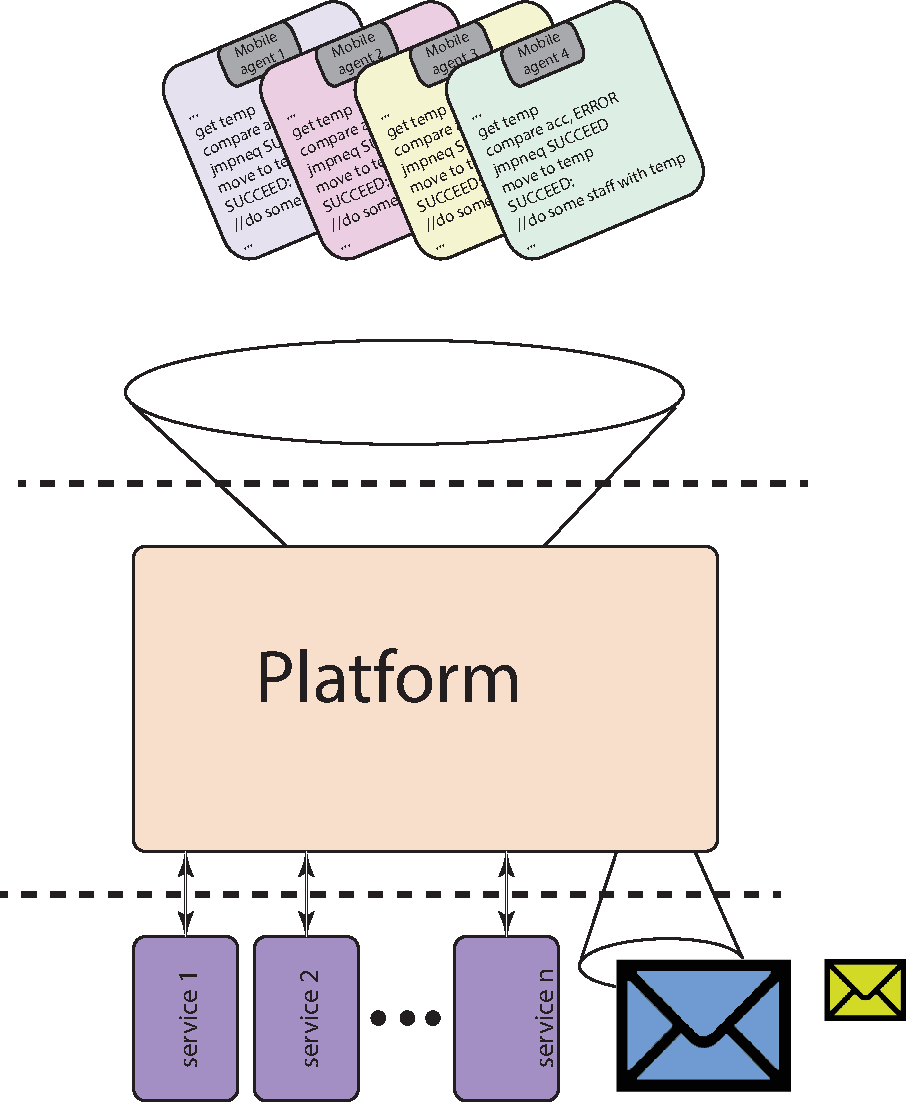
\includegraphics[height=2in]{img/overview_2-eps-converted-to.pdf}

\end{columns}
\end{frame}

\subsection{Agents}
\begin{comment}
\begin{frame}
	\frametitle{Agent language that support:}
	\begin{itemize}
	\item Arithmetical operations, branching and looping
	\item Message exchange
	\item Replication and code mobility
	\end{itemize}
% 	\framesubtitle{}

\end{frame}
\end{comment}

\begin{frame}
	\frametitle{Agents}
\includegraphics<1>[width=4in]{img/agent-1-eps-converted-to.pdf}
\includegraphics<2>[width=4in]{img/agent-2-eps-converted-to.pdf}
\includegraphics<3>[width=4in]{img/agent-3-eps-converted-to.pdf}
\includegraphics<4>[width=4in]{img/agent-4-eps-converted-to.pdf}	
% 	\framesubtitle{}

\end{frame}

\subsection{Platform}
\begin{frame}
	\frametitle{Platform}
% 	\framesubtitle{}
\begin{center}
\includegraphics<1>[scale=0.29]{img/plat1} 
\end{center}



\end{frame}

\subsubsection{Scheduler}
\begin{frame}
	\frametitle{Scheduler}
% 	\framesubtitle{}

\begin{center}
\includegraphics<1>[scale=0.27]{img/plat2} 
\end{center}

\end{frame}


\subsubsection{Execution Layer}
\begin{frame}
	\frametitle{Execution Layer}
% 	\framesubtitle{}
\begin{center}
\includegraphics<1>[scale=0.29]{img/plat3} 
\end{center}


\end{frame}


\subsection{Communication Protocol}

\begin{frame}
  \frametitle{Protocol Design}
    \begin{block}{Requirements}
      \begin{description}
        
      \item Local and remote communication 
        \begin{itemize}
          \item bridging layers            
        \end{itemize}
      \item Sending agent code 
        \begin{itemize}
        \item possibly large size            
        \end{itemize}
      \item Sending application data
        \begin{itemize}
        \item implicit time information            
        \end{itemize}
      \end{description}
    \end{block}
\end{frame}

\begin{frame}
  \frametitle{Network Infrastructure}
  \begin{figure}
    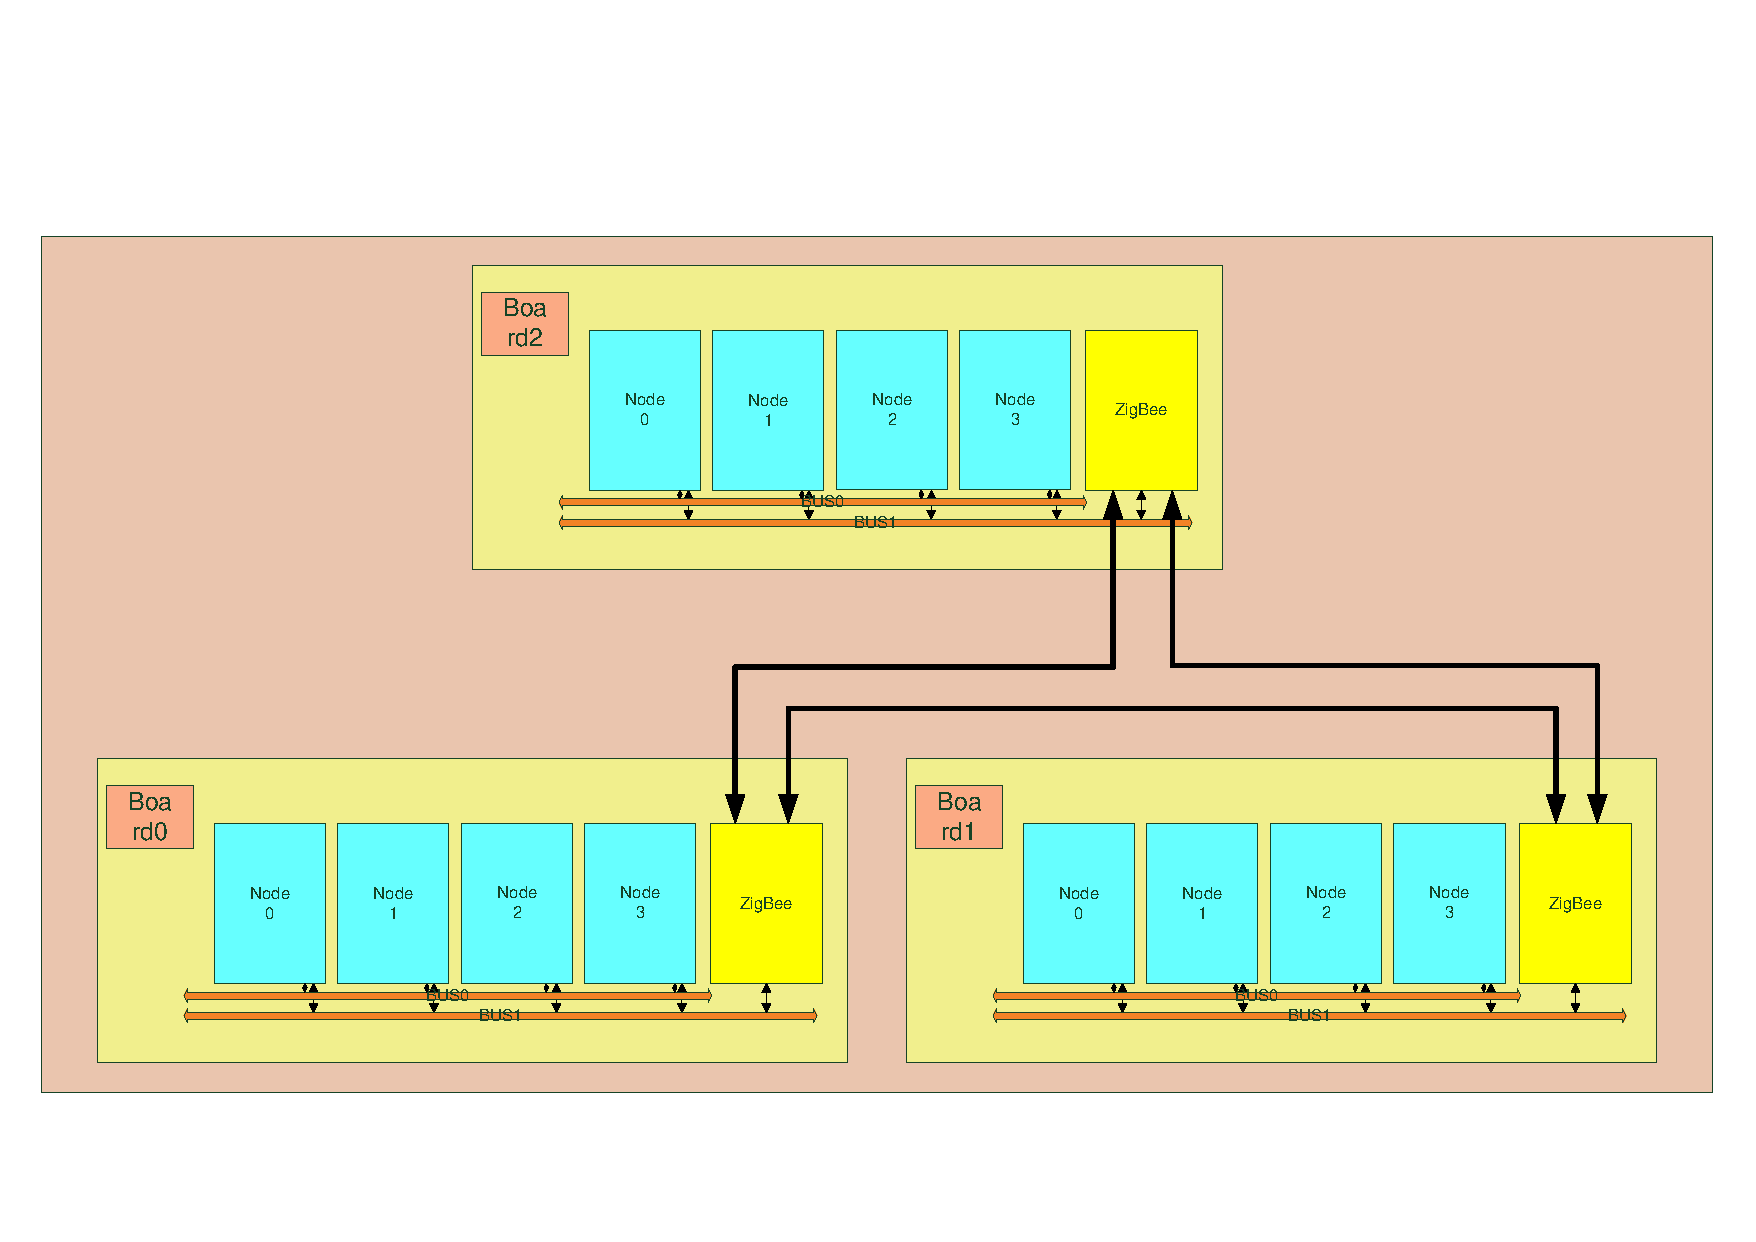
\includegraphics[width=0.9\textwidth]{img/zigbee.pdf}
  \end{figure}
\end{frame}

\begin{frame}
  \frametitle{Protocol Design cont.}
    \begin{block}{Design Principles}
      \begin{description}
      \item Layered design
        \begin{itemize}
          \item Low level - CSMA/CA
          \item High Level - Routing
        \end{itemize}
      \item Composability with \emph{Zigbee} 
        \begin{itemize}
          \item \emph{IEEE 802.15.4}
        \end{itemize}
      \item \emph{Fairness} in network access 
      \item Acknowledgement and retry  
        \begin{itemize}
        \item \emph{Unreliable network}
        \item \emph{Congestion avoidance}
        \item \emph{Complexity - e.g. TCP}
        \end{itemize}        
      \end{description}
    \end{block}
\end{frame}

\begin{frame}
  \frametitle{Transmission Layers}
  \begin{figure}
    \includegraphics<1>[width=0.35\textwidth]{img/packet-low-level.png} 
    \caption{Low Level Datagram}
  \end{figure}              

  \begin{figure}
    \includegraphics<1>[width=0.35\textwidth]{img/packet-upper-level.png}
    \caption{High Level Datagram}
  \end{figure}              

\end{frame}


\begin{frame}
  \frametitle{Network Configuration}
  \begin{figure}
    \includegraphics<1>[width=0.6\textwidth]{img/mesh-routing1.png} 
    \caption{Zigbee Mesh Network}
  \end{figure}
\end{frame}

\begin{frame}
  \frametitle{Zigbee Network Configuration}
  \framesubtitle{Rerouting Example}
  \begin{figure}
    \includegraphics<1>[width=0.6\textwidth]{img/mesh-routing2.png} 
    \caption{Network after rerouting}
  \end{figure}
  \begin{tabular}{llll}
    
\includegraphics[height=0.1in]{img/pink.png} & Network Coordinator & 
\includegraphics[height=0.1in]{img/blue} & Failed Node
 \\
    
\includegraphics[height=0.1in]{img/green} & Network Router & 
\includegraphics[height=0.1in]{img/route} & Message Route 
\\
  \end{tabular}
\end{frame}

  

\section{Project management}
\begin{frame}
	\frametitle{Milestones}
\begin{tabular}{ll}

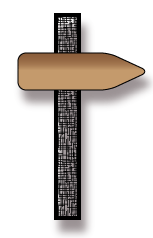
\includegraphics[height=0.3in]{img/milestone_03} & Phase 1. Product outline and information gathering\\
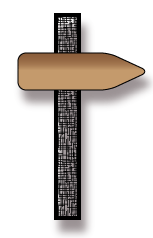
\includegraphics[height=0.3in]{img/milestone_03} & Phase 2. Application requirements and specification\\
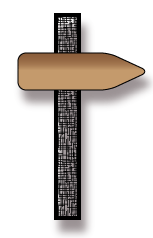
\includegraphics[height=0.3in]{img/milestone_03} & Phase 3. Implementation\\
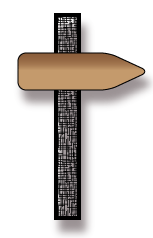
\includegraphics[height=0.3in]{img/milestone_03} & Phase 4. Validation and analysis\\
\end{tabular}

% 	\framesubtitle{}

\end{frame}

\begin{frame}
	\frametitle{Gantt diagram}

\begin{center}
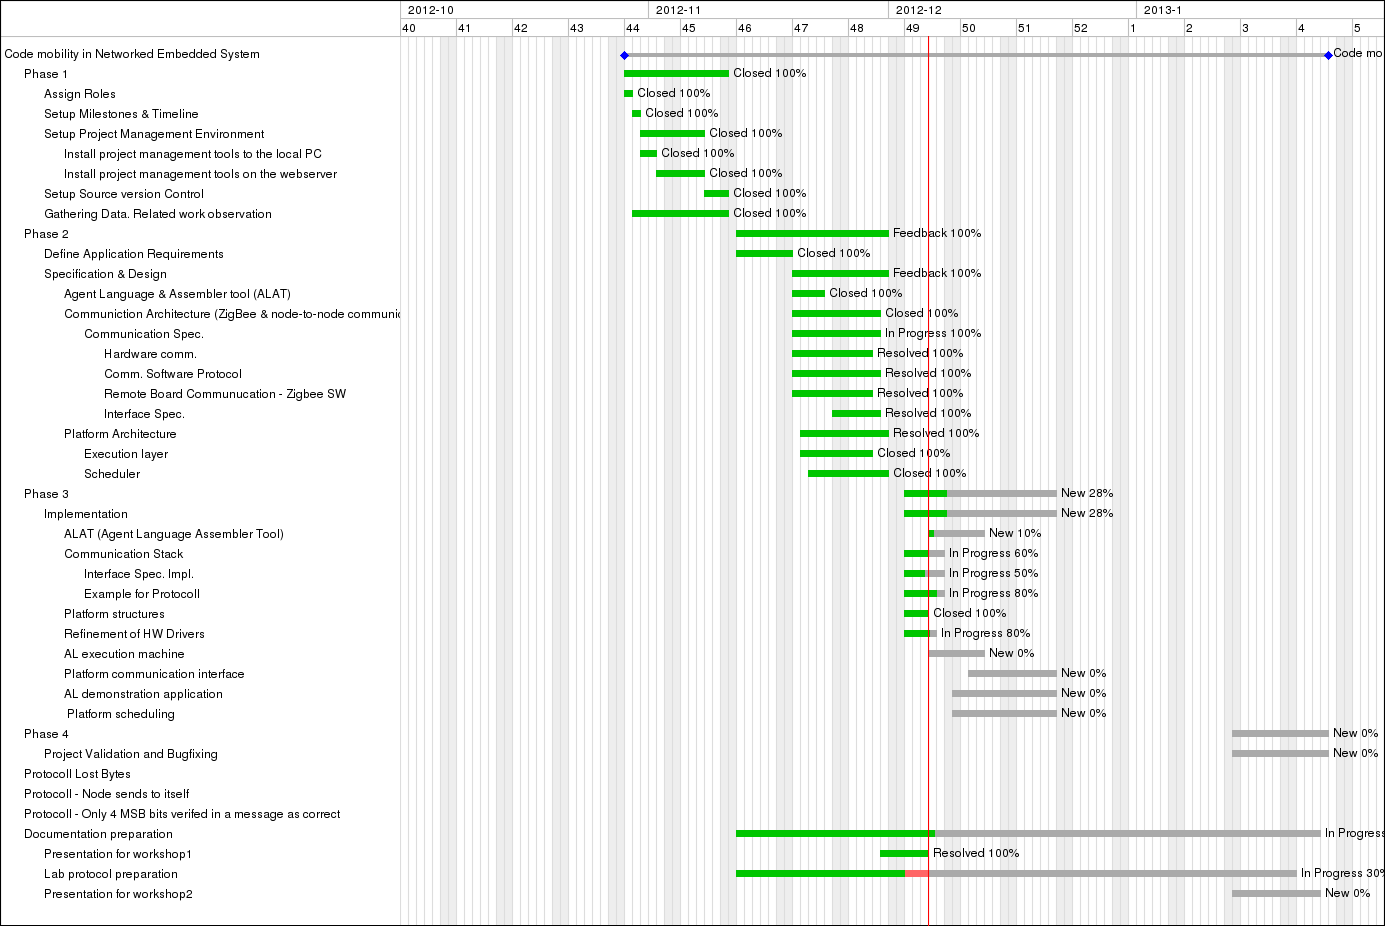
\includegraphics[height=2.7in]{img/gantt}

\end{center}
\end{frame}


\begin{frame}
	\frametitle{Workpackages}
% 	\framesubtitle{}
\scalebox{0.6}{
	\begin{tabular}{lllll}
	 & Name & Interdependencies & Dates & Deliverables\\\hline
	WP1 & Documentation & all &25.10.12 - 15.01.13 & D1.1 Lab protocol\\\hline
	    & 			&	&			& D1.2 specification\\\hline
	    & 			&	&			& D1.3 workshop1\\\hline
	    &			&	&			& D1.4 workshop2\\\hline
	WP2 & Adaption of drivers & 	& 5.12 - 15.12		& D2.1 hardware drivers\\\hline
	WP3 & Agent language tool &     & 6.12 - 10.12 		& D2.1 Agent language assembler tool\\\hline
	WP4 & Communication     & D2.1	& 			& Protocol\\\hline
	WP5 & Platform		& WP3, WP4	& 10.12 - 21.12 & D3.1 Platform \\\hline
	\end{tabular}
}
\end{frame}

\section{Tools}

\begin{frame}
	\frametitle{Tools}

\begin{tabular}{lcl}

Version control & 
\includegraphics[width=0.07\textwidth]{img/gitlogo} & git\\
Documentation \& code repository & 
\includegraphics[width=0.07\textwidth]{img/github-logo} & github\\
File sharing & 
\includegraphics[width=0.1\textwidth]{img/aws-logo} & amazon s3\\
Project management & 
\includegraphics[width=0.07\textwidth]{img/redmine-logo} & redmine\\
		& \multicolumn{2}{l}{\tiny{\href{http://nes2012group4.herokuapp.com/}{http://nes2012group4.herokuapp.com/}}}\\
%Code generation & 
\includegraphics[width=0.07\textwidth]{img/scade-logo} & SCADE\\
IDE & & Eclipse\\
Editors & 
\includegraphics[width=0.07\textwidth]{img/emacs-logo} & Emacs\\

\end{tabular}

\end{frame}


\begin{frame}
	\frametitle{References}
	\bibliography{presentation}
	\bibliographystyle{alpha}

\end{frame}


\begin{frame}
	\frametitle{Questions}

\end{frame}

\begin{frame}
	

\end{frame}

\begin{frame}
	\frametitle{Roles}
\begin{center}
\scalebox{0.6}{	
	\begin{tabular}{ll}
%	\textbf{Role}		& \textbf{Responsibilies}\\\hline
	\hline
	\multicolumn{2}{c}{Konstantin Selyunin}\\
	Project manager & internal coordination\\
			& defining tasks\\
			& control meeting deadlines\\\hline
	\multicolumn{2}{c}{Igor Pelesi\'c}\\
	System architect & technical decisions\\
			 & determine technical part of the project\\\hline
	\multicolumn{2}{c}{Miljenko Jakovljevi\'c}\\
	Documentation responsible & Lab protocol\\
				  & documentation decisions\\
	\end{tabular}
}
\end{center}
\end{frame}

\begin{comment}
\begin{frame}
	\frametitle{Goals}
Our goals:
	\begin{itemize}
		\item Design, implement and evaluate code mobility system on ESE Board
		\item Hardware drivers \& mobile agents \& communication
		\item Master project management skills
	\end{itemize}
\end{frame}


\begin{frame}
	\frametitle{Use cases}

\end{frame}


\begin{frame}
	\frametitle{Risk management}

\end{frame}

\begin{frame}
	\frametitle{High-level agent language}

\end{frame}
\end{comment}
% End of document
\end{document}
